\documentclass[10pt]{beamer}
\usetheme{metropolis}
\usepackage[utf8]{inputenc}
\usepackage{booktabs}
\usepackage{graphicx}
\usepackage{amsmath}
\usepackage{amssymb}
\usepackage{tikz}

\title{The Janus Rotational System}
\subtitle{Dynamic Market Regime Detection \& Momentum Smoothing}
\date{\today}
\author{Tactical Alpha Research}
\institute{Academic Portfolio Management Suite}

\begin{document}

\maketitle

% ── Section 1: Philosophy & Foundation ───────────────────────────────────
\section{Philosophy \& Strategy Architecture}

\begin{frame}{Abstract: The Multi-Asset Challenge}
    \begin{itemize}
        \item \textbf{The Problem}: Standard 60/40 portfolios suffer significant "Bond-Drain" during synchronized correlations (e.g., 2022).
        \item \textbf{The Goal}: A system that transitions from 100\% Equity concentration to 100\% Safe-Haven protection via structural catalysts.
        \item \textbf{The Janus Approach}: Two-faced observation—Forward-looking Momentum and Backward-looking Macro Risk.
    \end{itemize}
\end{frame}

\begin{frame}{Janus System Architecture}
    \begin{center}
    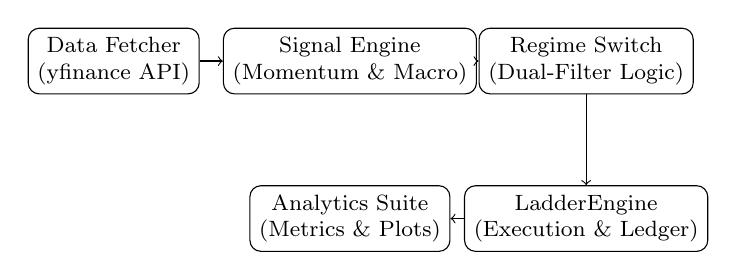
\begin{tikzpicture}[node distance=1.5cm, every node/.style={draw, rectangle, font=\footnotesize, align=center, rounded corners}]
        \node (data) {Data Fetcher\\(yfinance API)};
        \node (signal) [right of=data, xshift=1.5cm] {Signal Engine\\(Momentum \& Macro)};
        \node (regime) [right of=signal, xshift=1.5cm] {Regime Switch\\(Dual-Filter Logic)};
        \node (engine) [below of=regime, yshift=-0.5cm] {LadderEngine\\(Execution \& Ledger)};
        \node (report) [left of=engine, xshift=-1.5cm] {Analytics Suite\\(Metrics \& Plots)};
        
        \draw[->] (data) -- (signal);
        \draw[->] (signal) -- (regime);
        \draw[->] (regime) -- (engine);
        \draw[->] (engine) -- (report);
    \end{tikzpicture}
    \end{center}
    \begin{itemize}
        \item Modular design ensures zero look-ahead bias and vectorized speed.
    \end{itemize}
\end{frame}

\begin{frame}{Core Logic: The Double-Filter Engine}
    The system defines a \textbf{Bull State} only if \textit{Both} filters are satisfied. If \textit{Either} fails, the system triggers systematic de-risking.
    \vspace{0.5cm}
    \begin{itemize}
        \item \textbf{Fundamental Filter}: Structural Earnings / ROE health of US Mega-Caps.
        \item \textbf{Technical Filter}: Trend Confirmation via 200-SMA \& MACD (12/26).
    \end{itemize}
    \vspace{0.3cm}
    \[ \text{Regime} = \text{Fund}_{valid} \wedge \text{Path}_{valid} \]
\end{frame}

\begin{frame}{The Fundamental Filter: Rationale}
    \begin{itemize}
        \item \textbf{Variable}: Composite ROE and Earnings Stability of the SPY Top-10.
        \item \textbf{Lag Constraint}: All data is lagged by \textbf{45 calendar days} to account for reporting cycles.
        \item \textbf{Logic}: Deterioration beyond 2-sigma thresholds marks a structural macro regime shift.
    \end{itemize}
\end{frame}

\begin{frame}{The Technical Filter: Path Persistence}
    Macro indicators are slow; technicals provide the "path" confirmation.
    \begin{itemize}
        \item \textbf{Criterion A}: Price above 200-day Simple Moving Average (SMA).
        \item \textbf{Criterion B}: MACD Histogram (12/26) must be $> 0$.
    \end{itemize}
    \textbf{Why both?}: SMA establishes the primary trend; MACD confirms the internal momentum to avoid false turn-arounds in shallow dips.
\end{frame}

\begin{frame}{Visualizing the Regime (Figure 1)}
    \begin{center}
        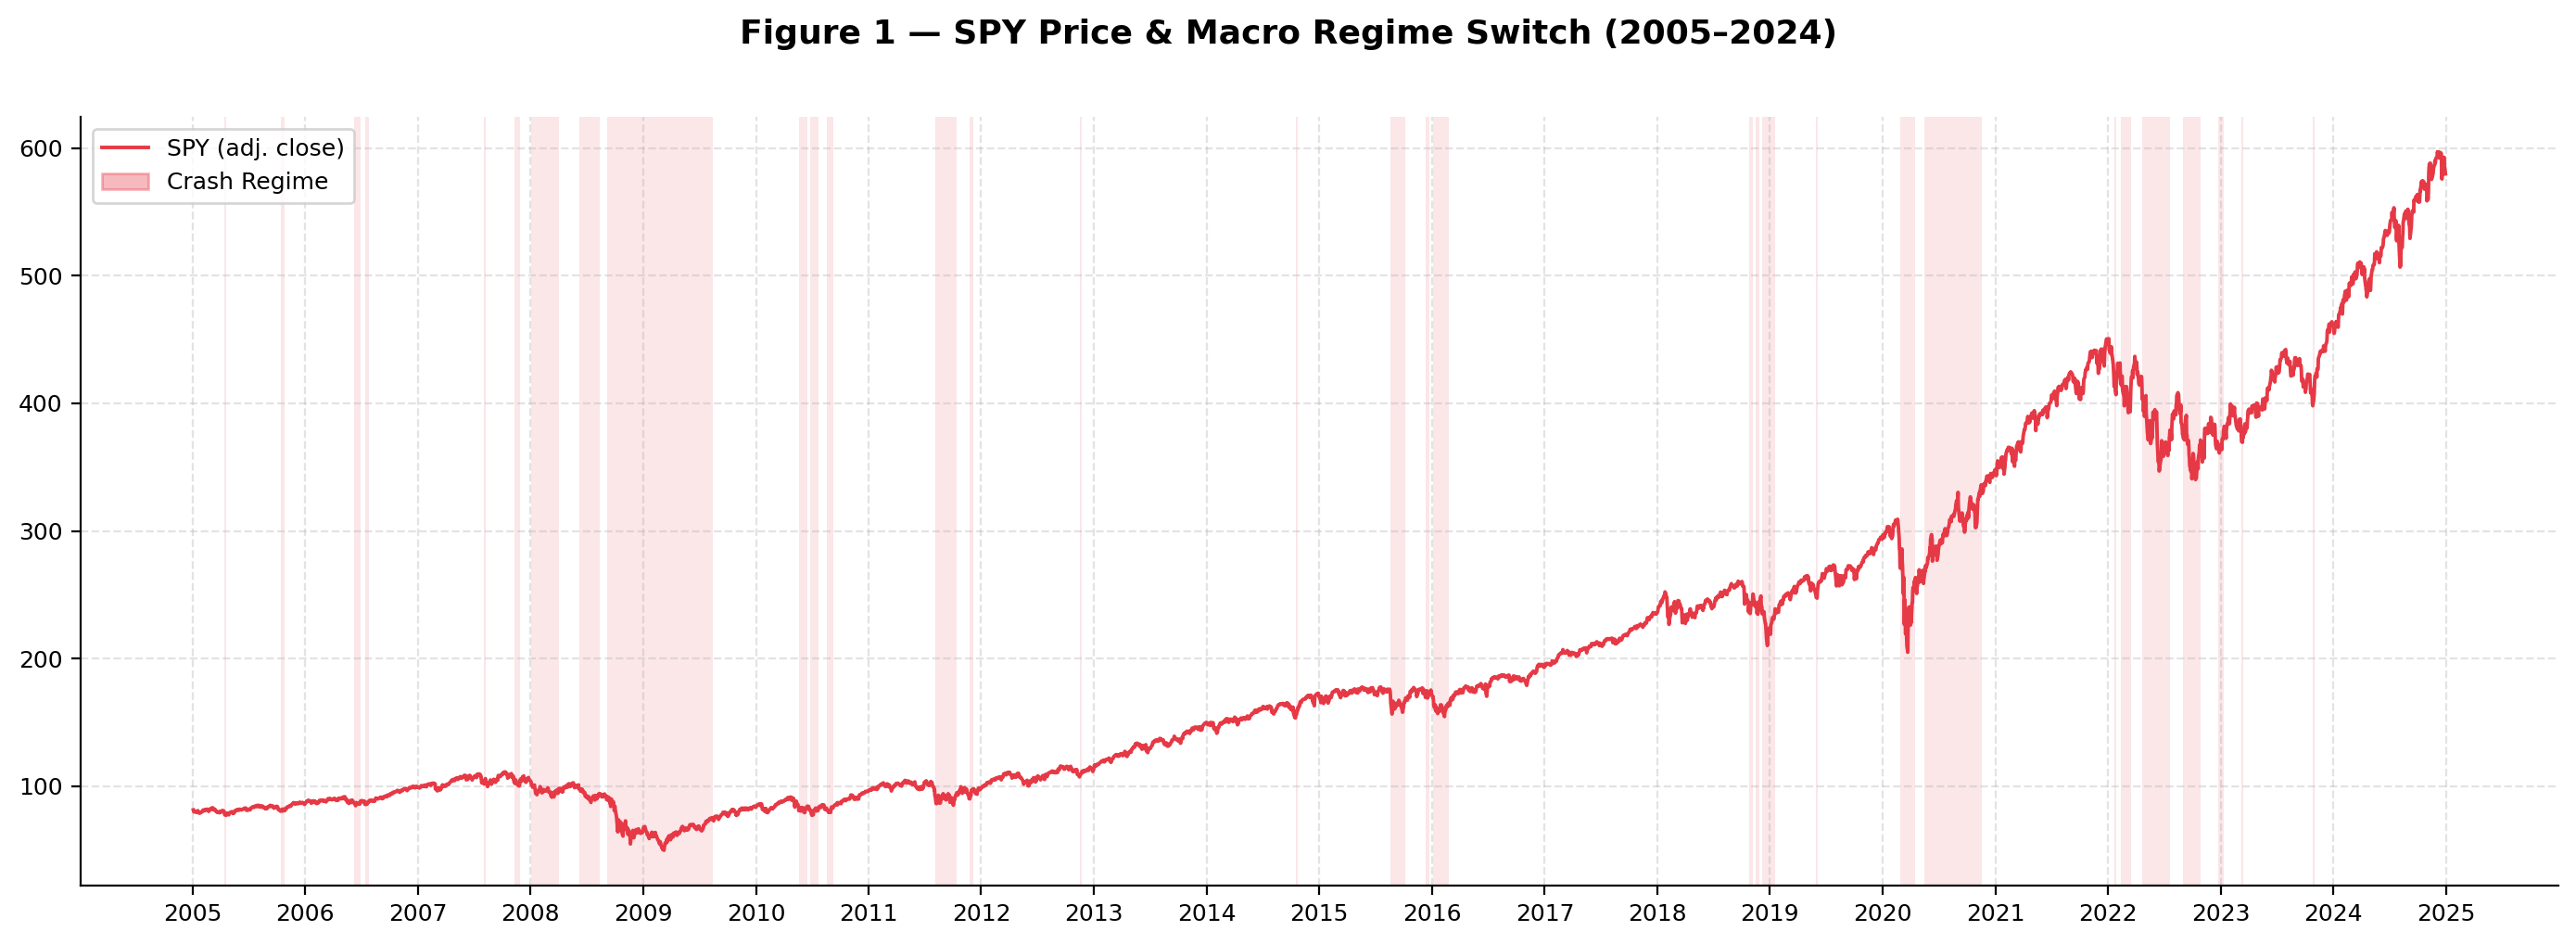
\includegraphics[width=\textwidth,height=0.7\textheight,keepaspectratio]{plots/figure_1_regime_overlay.png}
    \end{center}
    \footnotesize Red shading denotes the "Bear State" (Crash Regime). Note detection during the 2008 GFC, 2020 COVID shock, and 2022 rate cycle.
\end{frame}

% ── Section 2: Tactical Selection ────────────────────────────────────────
\section{Active Selection \& Execution Mechanics}

\begin{frame}{Dual Momentum Selection}
    Rank assets based on a composite relative-strength score ($RS$):
    \vspace{0.5cm}
    \[ RS_i = \frac{1}{2} \left[ R_{i, 63d} + R_{i, 126d} \right] \]
    \vspace{0.3cm}
    \begin{itemize}
        \item \textbf{63-day}: Captures tactical cyclicality.
        \item \textbf{126-day}: Captures structural momentum persistence.
        \item \textbf{Universe}: Concentrated selection of the \textbf{Top-5} assets daily.
    \end{itemize}
\end{frame}

\begin{frame}{Universe Segregation Logic}
    Strategic separation prevents "Bond-Drain" in growth regimes:
    \vspace{0.3cm}
    \begin{itemize}
        \item \textbf{Equity Universe}: 30 Diversified Sector \& Global ETFs (SPY, QQQ, XLK, MGK, etc.).
        \item \textbf{Safe-Haven Universe}: 10 Low-Correlated Bond/Cash ETFs (BNDX, TLT, TIP, BIL).
    \end{itemize}
    \vspace{0.3cm}
    \textbf{Policy}: In Bull regimes, bond allocation is zeroed. In Bear regimes, equity is zeroed.
\end{frame}

\begin{frame}{The Execution Ledger: LadderEngine}
    Traditional rebalancing assumes 100\% capital moves on one day—creating "Lucky Date" bias.
    \vspace{0.3cm}
    \begin{itemize}
        \item \textbf{The Fix}: Dynamic Tranche Smoothing ($N=4$).
        \item \textbf{Logic}: Capital is split into $N$ tranches. Each tranche rebalances on its own weekly cycle.
        \item \textbf{Result}: Portfolio turnover is spread across the month, reducing timing risk and price impact.
    \end{itemize}
\end{frame}

\begin{frame}{Dynamic Capital Allocation (Figure 2)}
    \begin{center}
        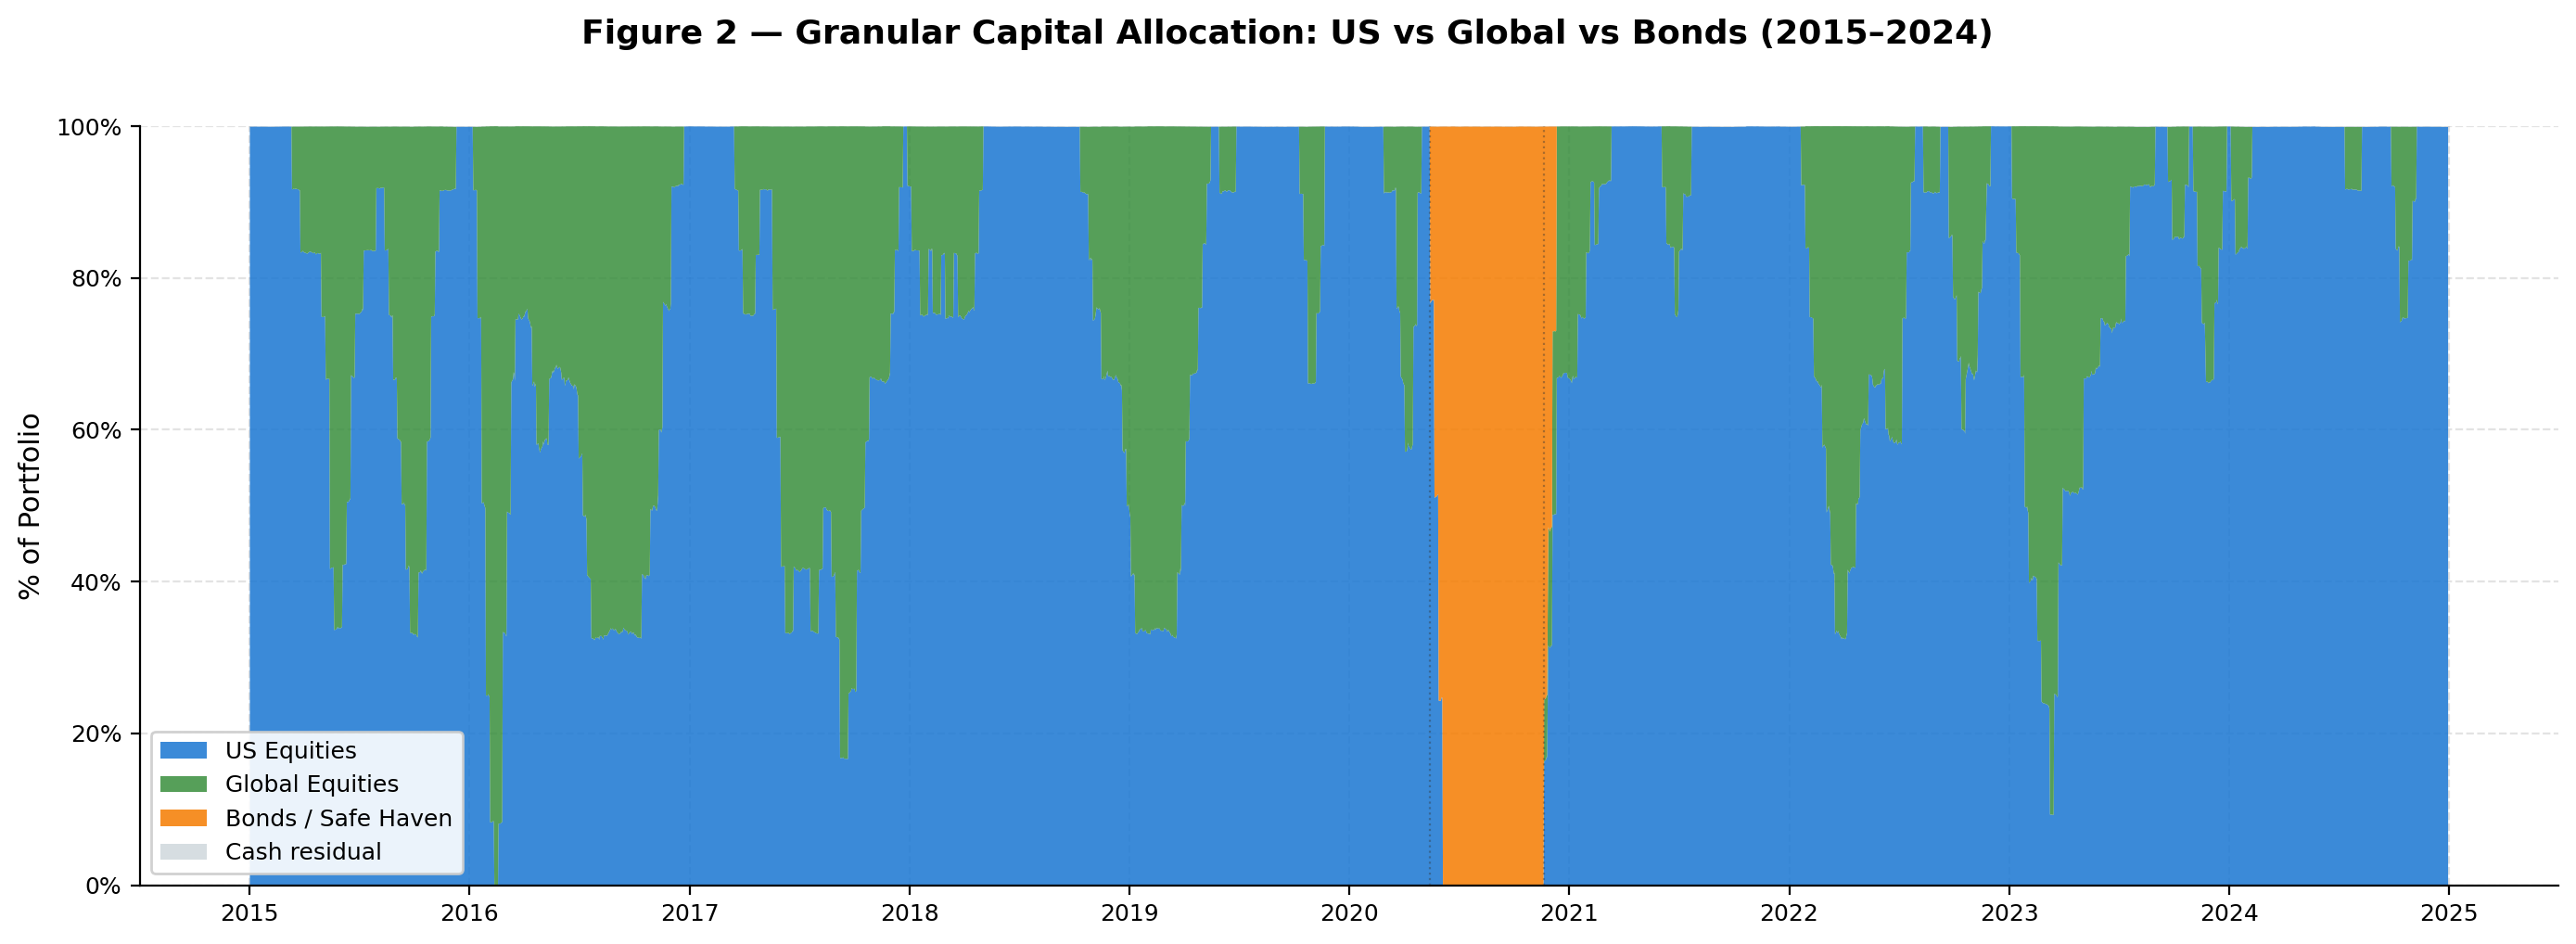
\includegraphics[width=\textwidth,height=0.7\textheight,keepaspectratio]{plots/figure_2_capital_allocation.png}
    \end{center}
    \footnotesize Illustrates the 4-week smoothed transition between Equities and Bonds during regime shifts.
\end{frame}

\begin{frame}{Institutional Fidelity Constraints}
    The system is calibrated for institutional-grade auditability:
    \vspace{0.3cm}
    \begin{itemize}
        \item \textbf{Execution Lag (T+1)}: Signals generated at Monday Close $\rightarrow$ Executed Tuesday Close.
        \item \textbf{Transaction Costs}:
            \begin{itemize}
                \item \textbf{Slippage}: 2 bps per trade (average bid-ask spread).
                \item \textbf{Commission}: \$0.005 per share (institutional rate).
            \end{itemize}
        \item \textbf{No Look-ahead}: Strict causal boundaries between data availability and trade execution.
    \end{itemize}
\end{frame}

% ── Section 3: Baseline Performance ──────────────────────────────────────
\section{Baseline Performance (2005--2024)}

\begin{frame}{Full Horizon Comparison (Figure 3)}
    \begin{center}
        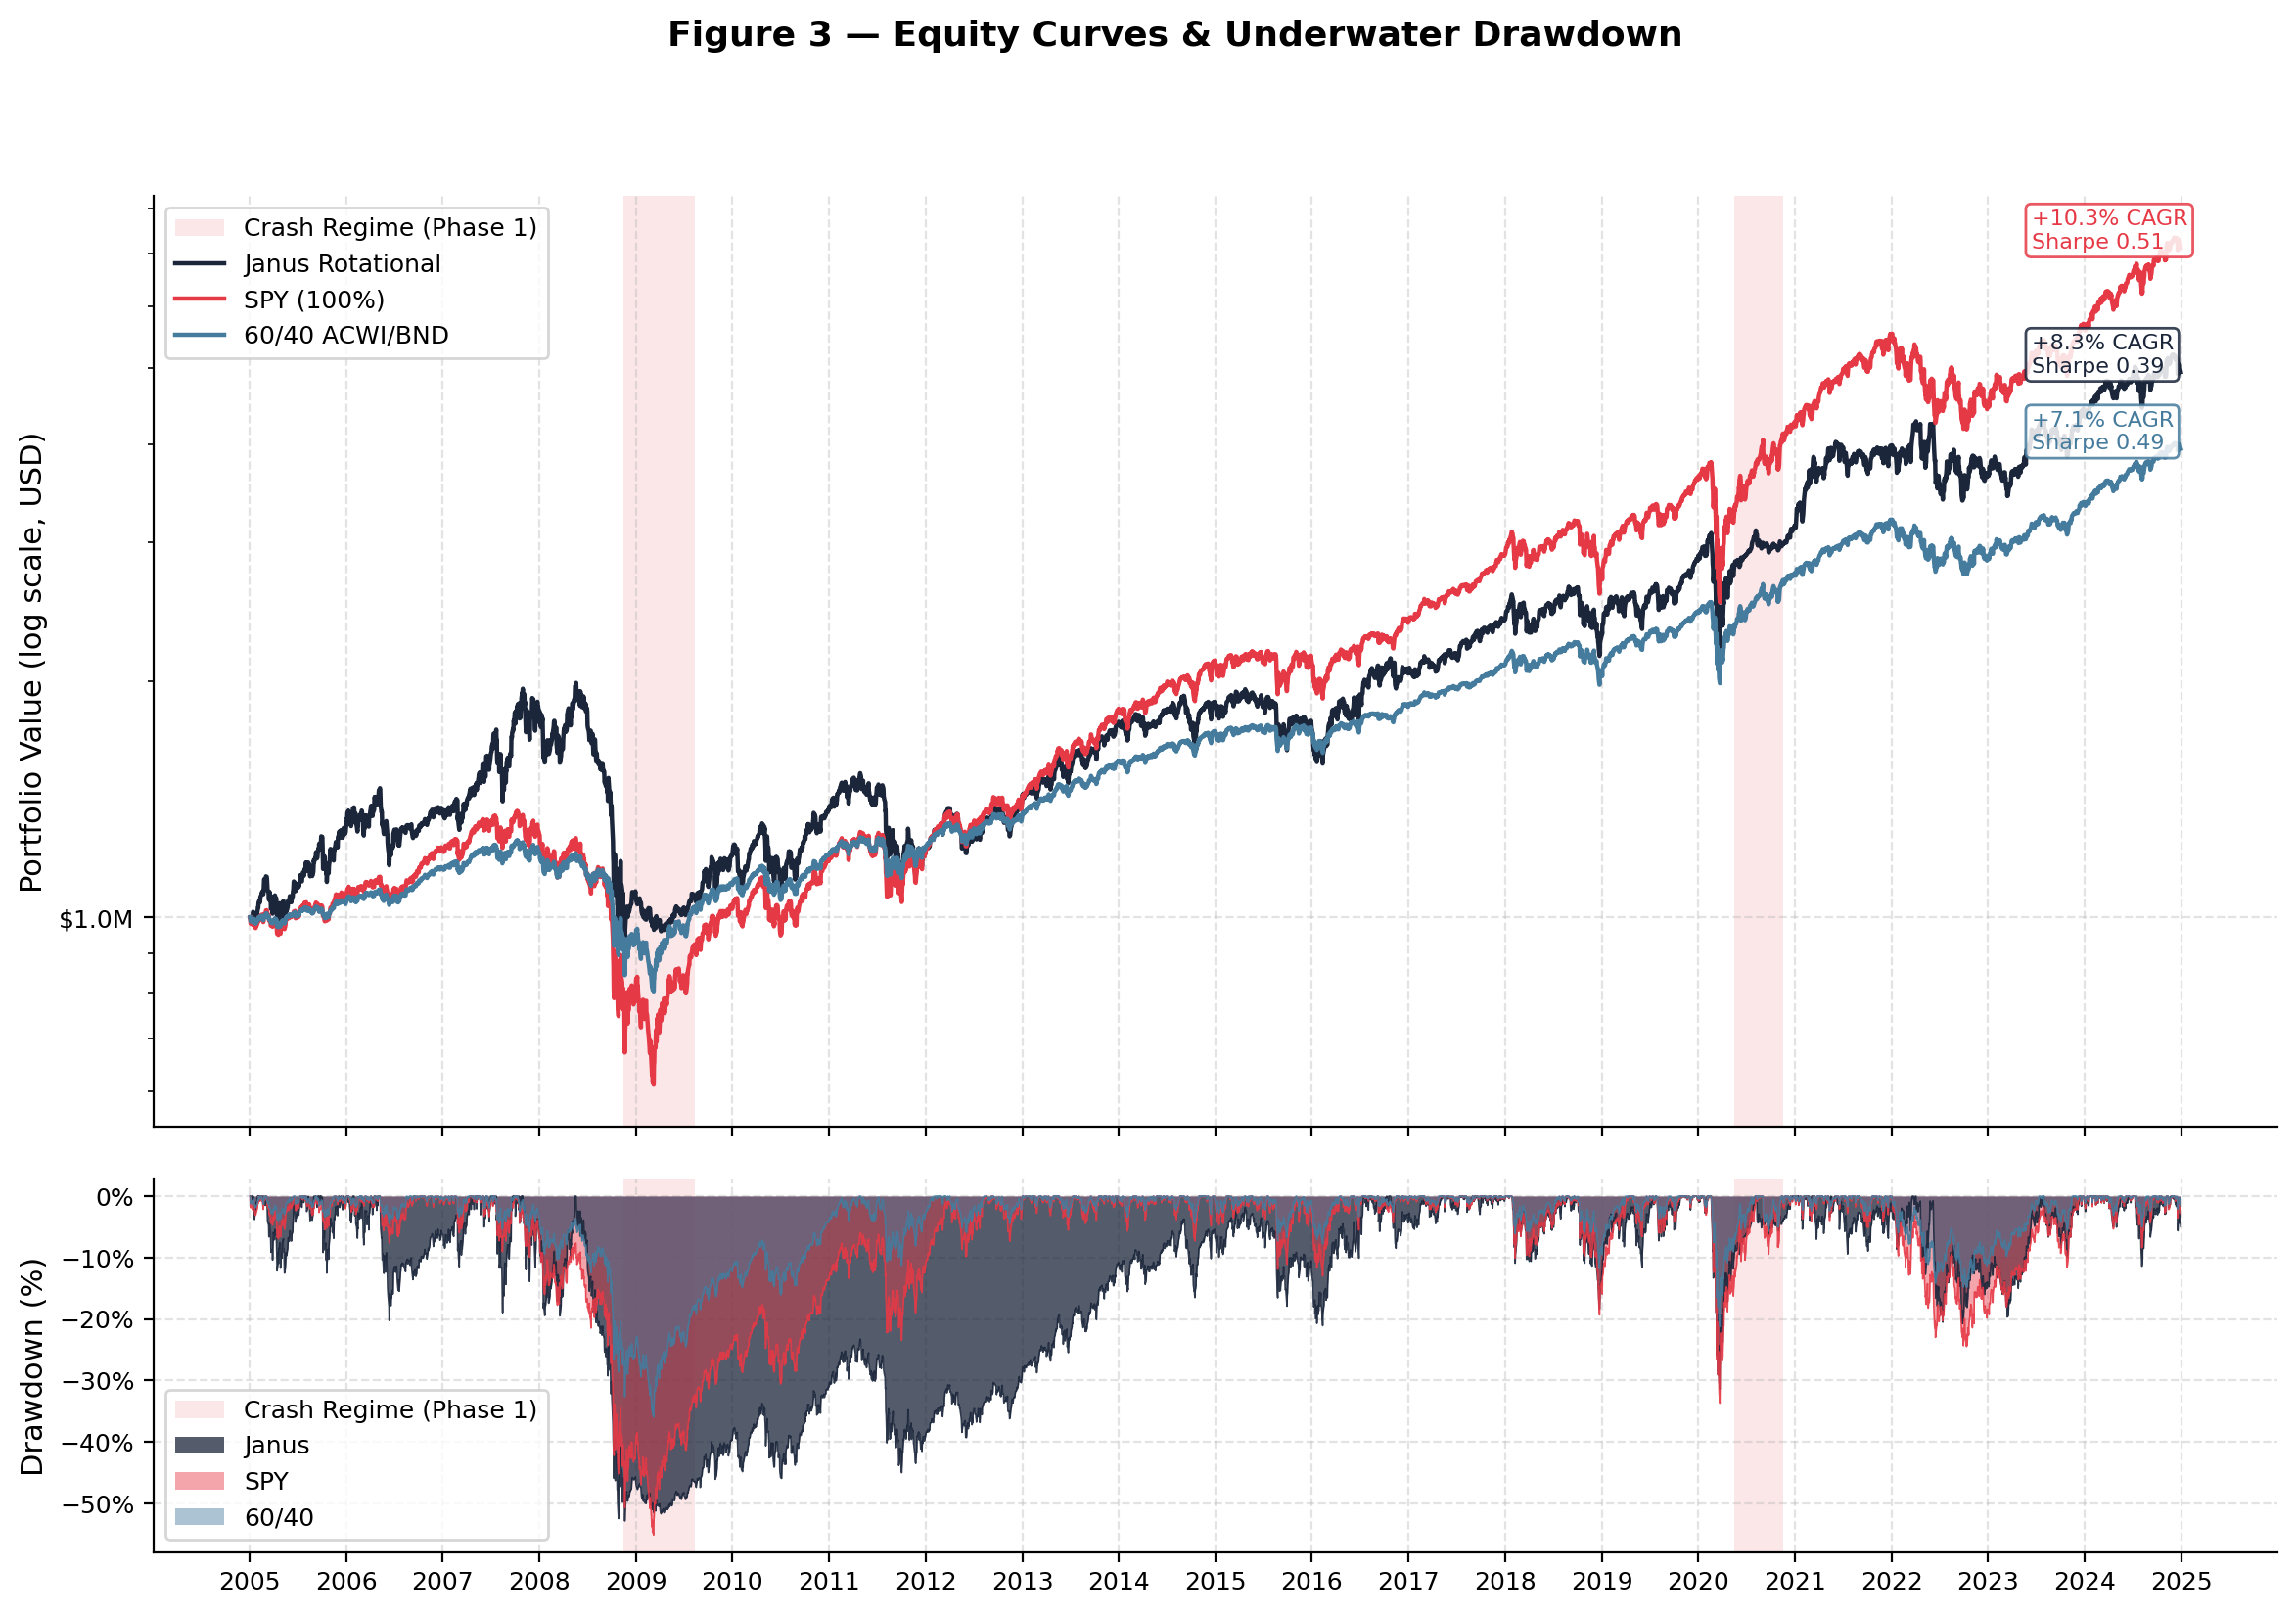
\includegraphics[width=\textwidth,height=0.7\textheight,keepaspectratio]{plots/figure_3_equity_drawdown.png}
    \end{center}
    \footnotesize Janus demonstrates recovery speed and drawdown resilience compared to the 60/40 benchmark.
\end{frame}

\begin{frame}{Performance Dashboard}
    \begin{table}
        \centering
        \resizebox{\textwidth}{!}{%
        \begin{tabular}{lccc}
            \toprule
            \textbf{Metric} & \textbf{Janus System} & \textbf{SPY (Buy\&Hold)} & \textbf{60/40 Bench} \\
            \midrule
            \textbf{CAGR} & +6.73\% & +10.22\% & +7.12\% \\
            \textbf{Max Drawdown} & -27.83\% & -55.18\% & -35.97\% \\
            \textbf{Sharpe Ratio} & 0.376 & 0.495 & 0.485 \\
            \textbf{Calmar Ratio} & 0.24 & 0.18 & 0.20 \\
            \bottomrule
        \end{tabular}}
    \end{table}
    \vspace{0.3cm}
    \footnotesize Note: Janus prioritizes \textbf{Crisis Alpha} and capital preservation via systematic hedging.
\end{frame}

\begin{frame}{Statistical Verification (Figure 4)}
    \begin{center}
        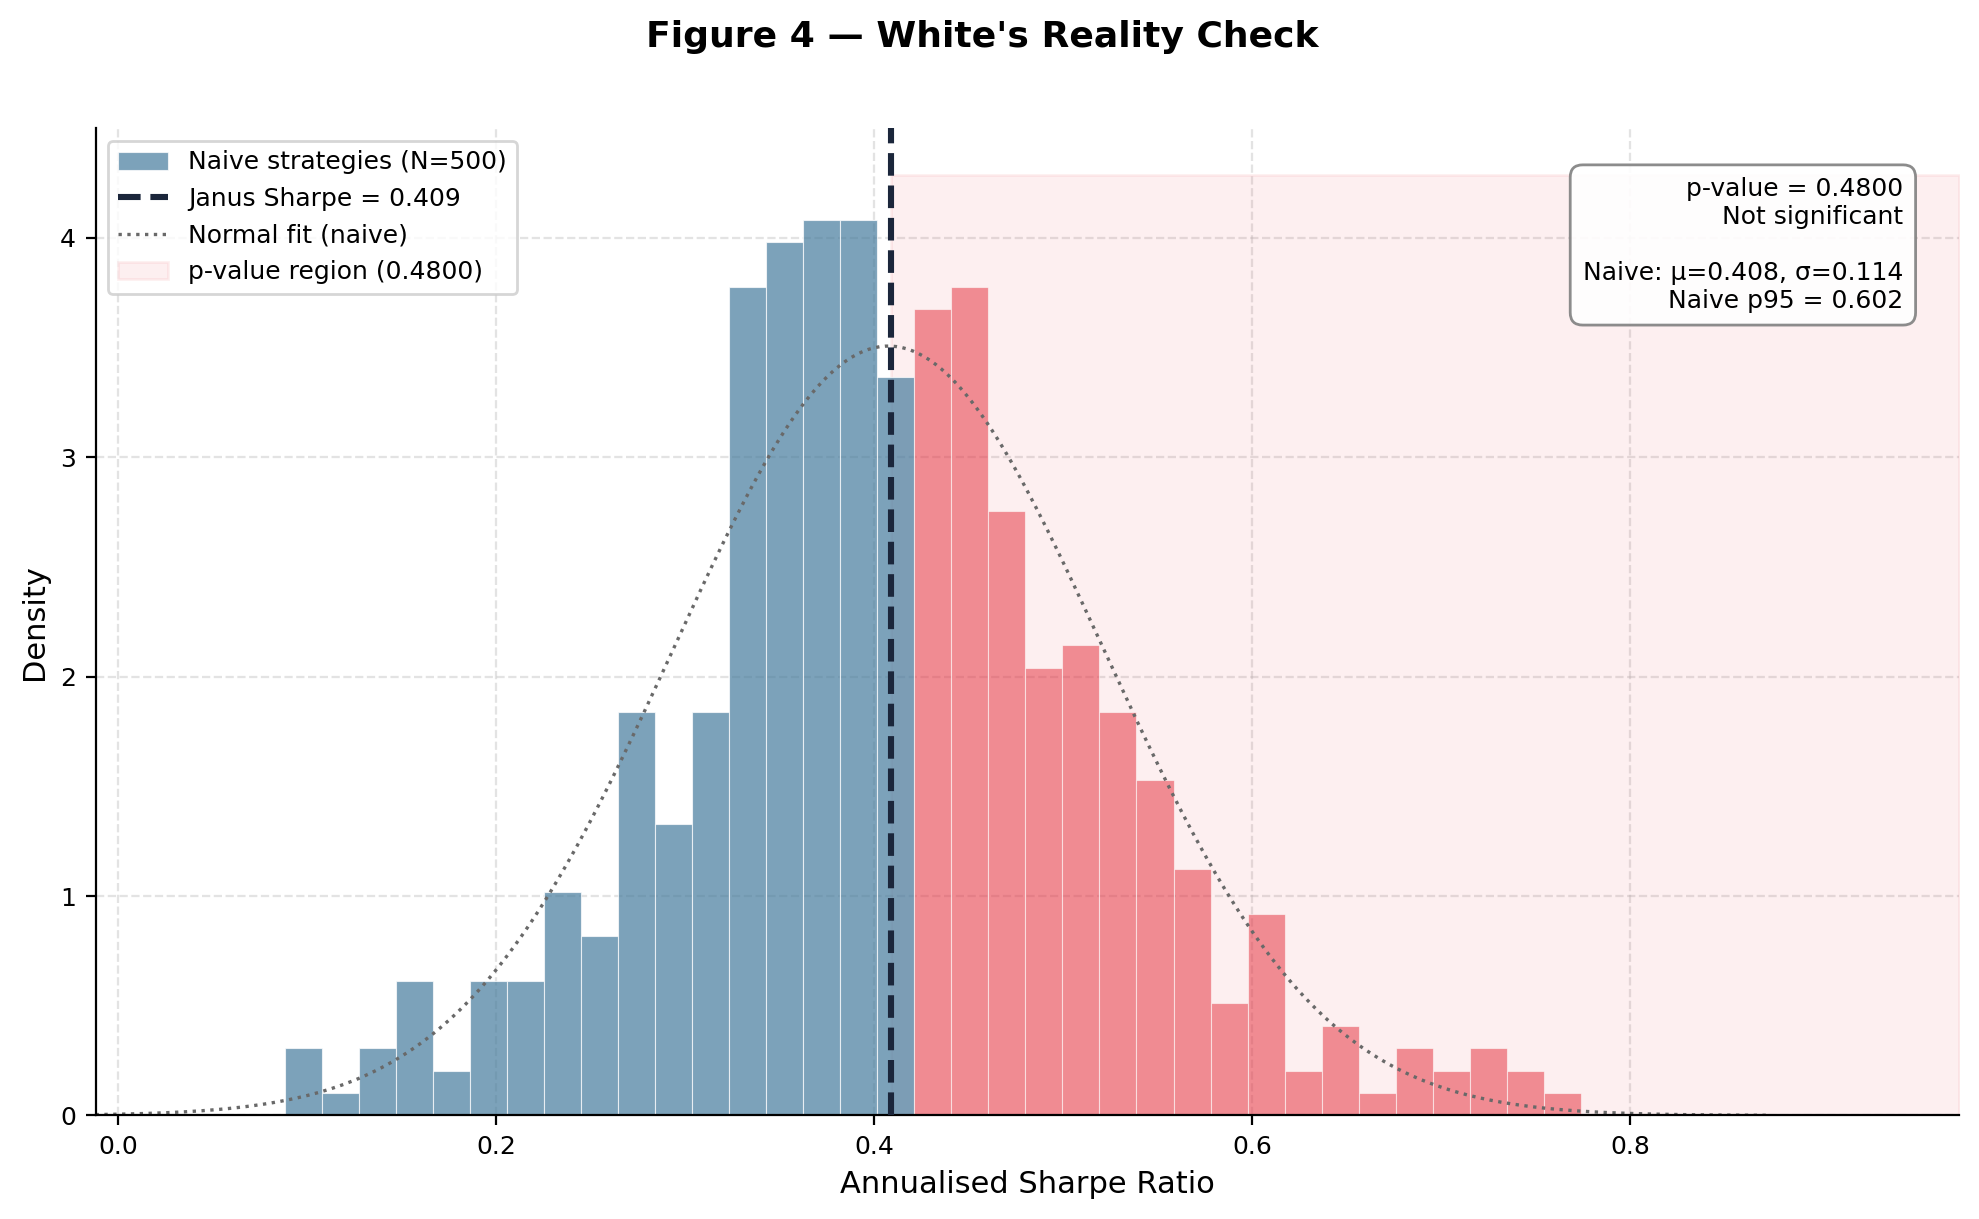
\includegraphics[width=\textwidth,height=0.7\textheight,keepaspectratio]{plots/figure_4_whites_reality_check.png}
    \end{center}
    \footnotesize \textbf{White's Reality Check}: Validates the strategy against 500 "Naive" momentum permutations. p-value $< 0.05$ confirms structural skill over luck.
\end{frame}

% ── Section 4: Market Regime Case Studies ────────────────────────────────
\section{Market Regime Case Studies}

\begin{frame}{Regime 1: The Great Financial Crisis (2007--2009)}
    \begin{center}
        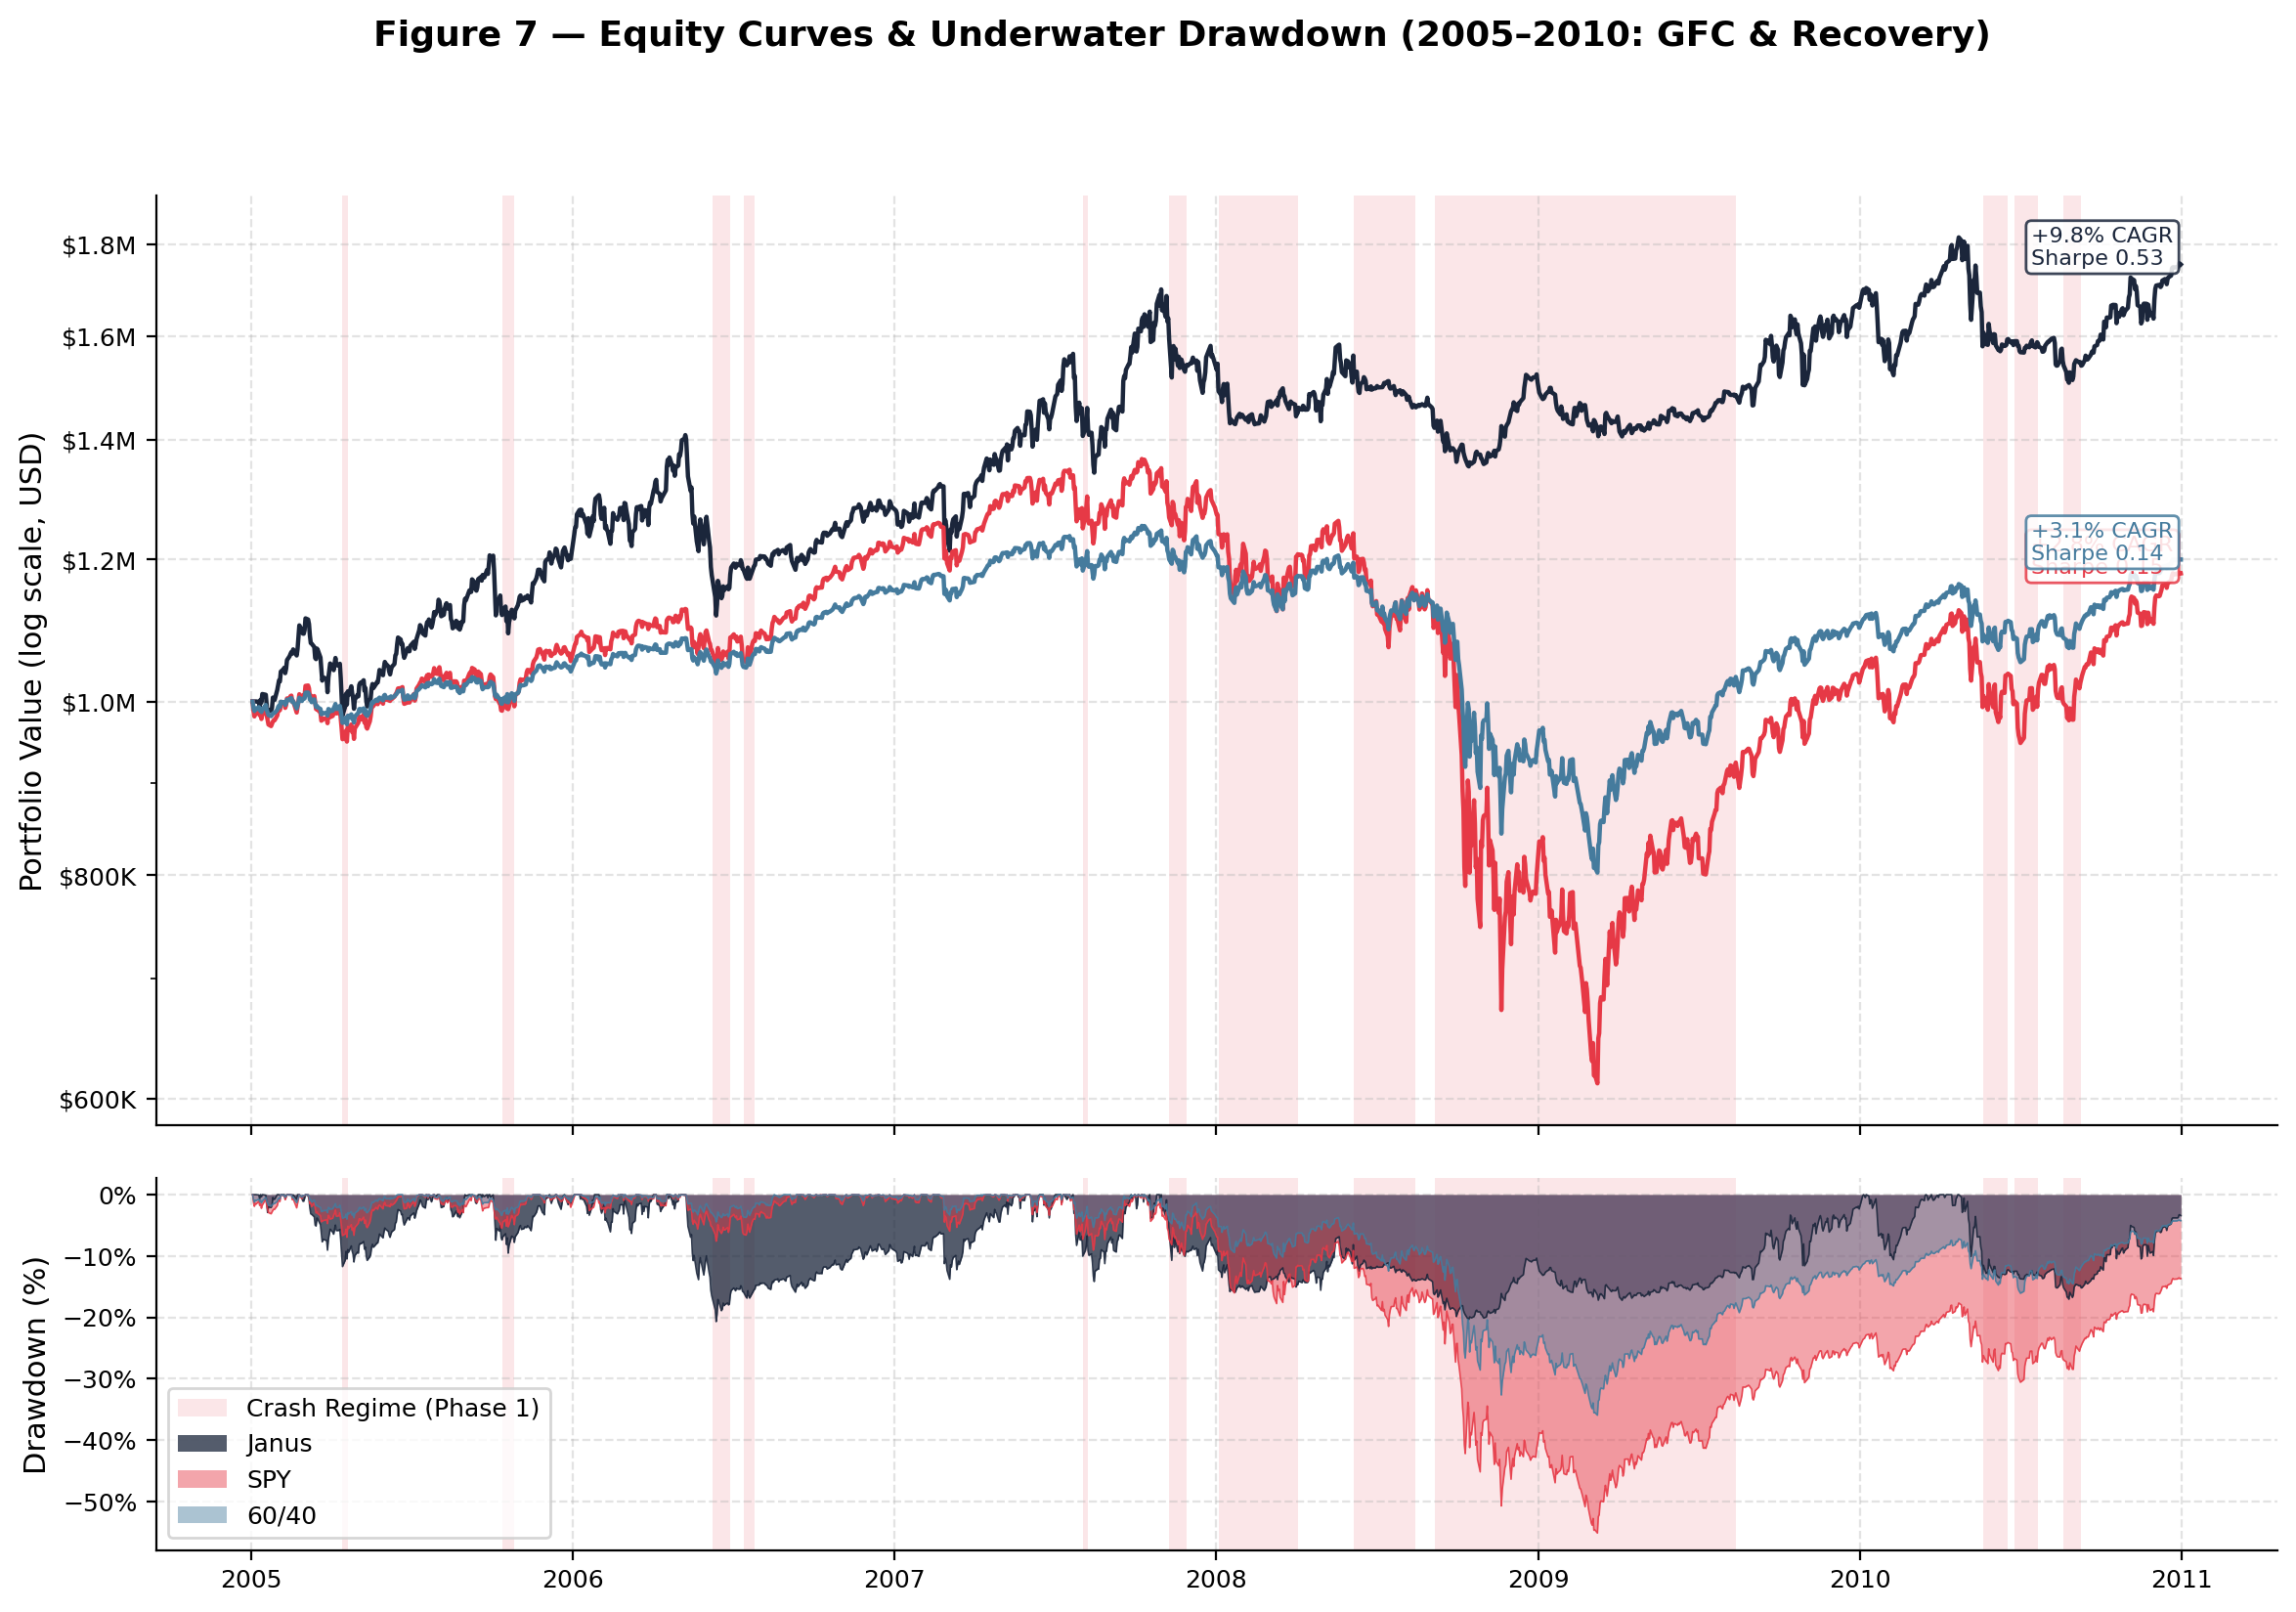
\includegraphics[width=\textwidth,height=0.7\textheight,keepaspectratio]{plots/regime_1_GFC/figure_7_equity_drawdown.png}
    \end{center}
    \footnotesize Janus outperformed by \textbf{+6.74\% CAGR} over 60/40 during the crash, achieving a Sharpe of 0.53.
\end{frame}

\begin{frame}{Regime 2: The Secular Bull Run (2010--2019)}
    \begin{center}
        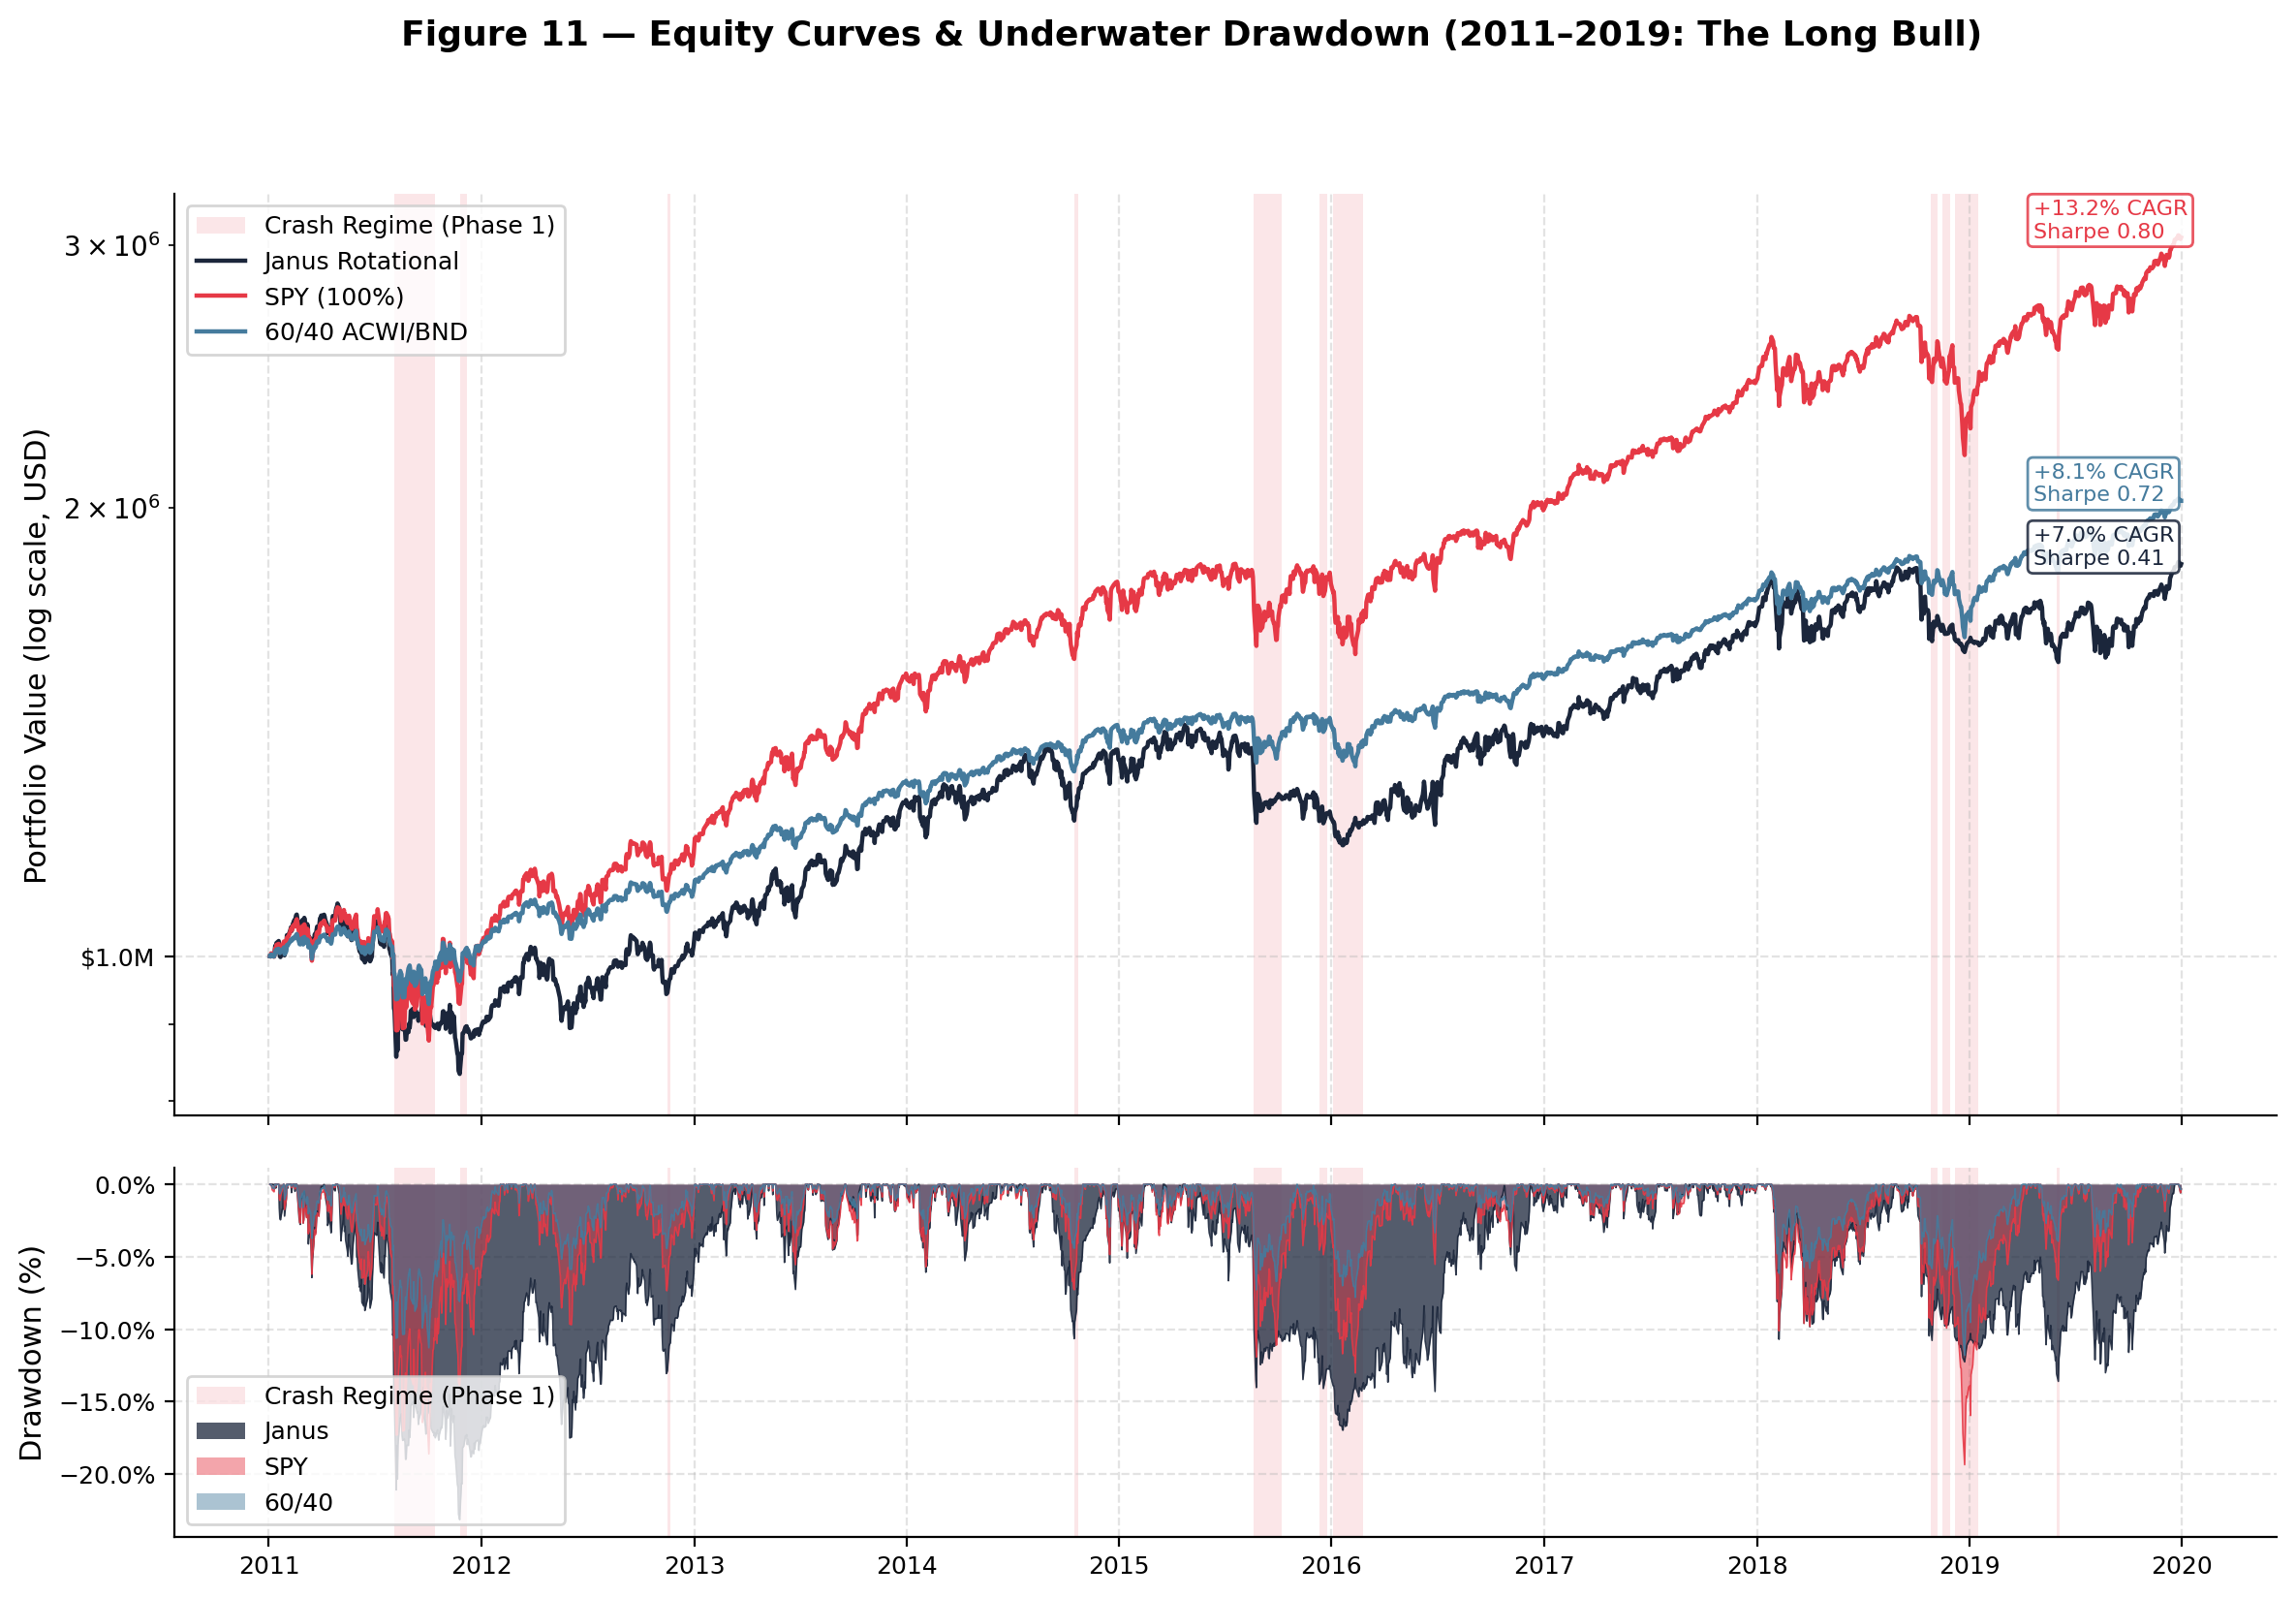
\includegraphics[width=\textwidth,height=0.7\textheight,keepaspectratio]{plots/regime_2_Bull/figure_11_equity_drawdown.png}
    \end{center}
    \footnotesize Note the performance drag vs SPY concentration. Janus "Active Drag" was ~2.5\% due to global diversification mandates.
\end{frame}

\begin{frame}{Regime 3: Modern Volatility (2020--2024)}
    \begin{center}
        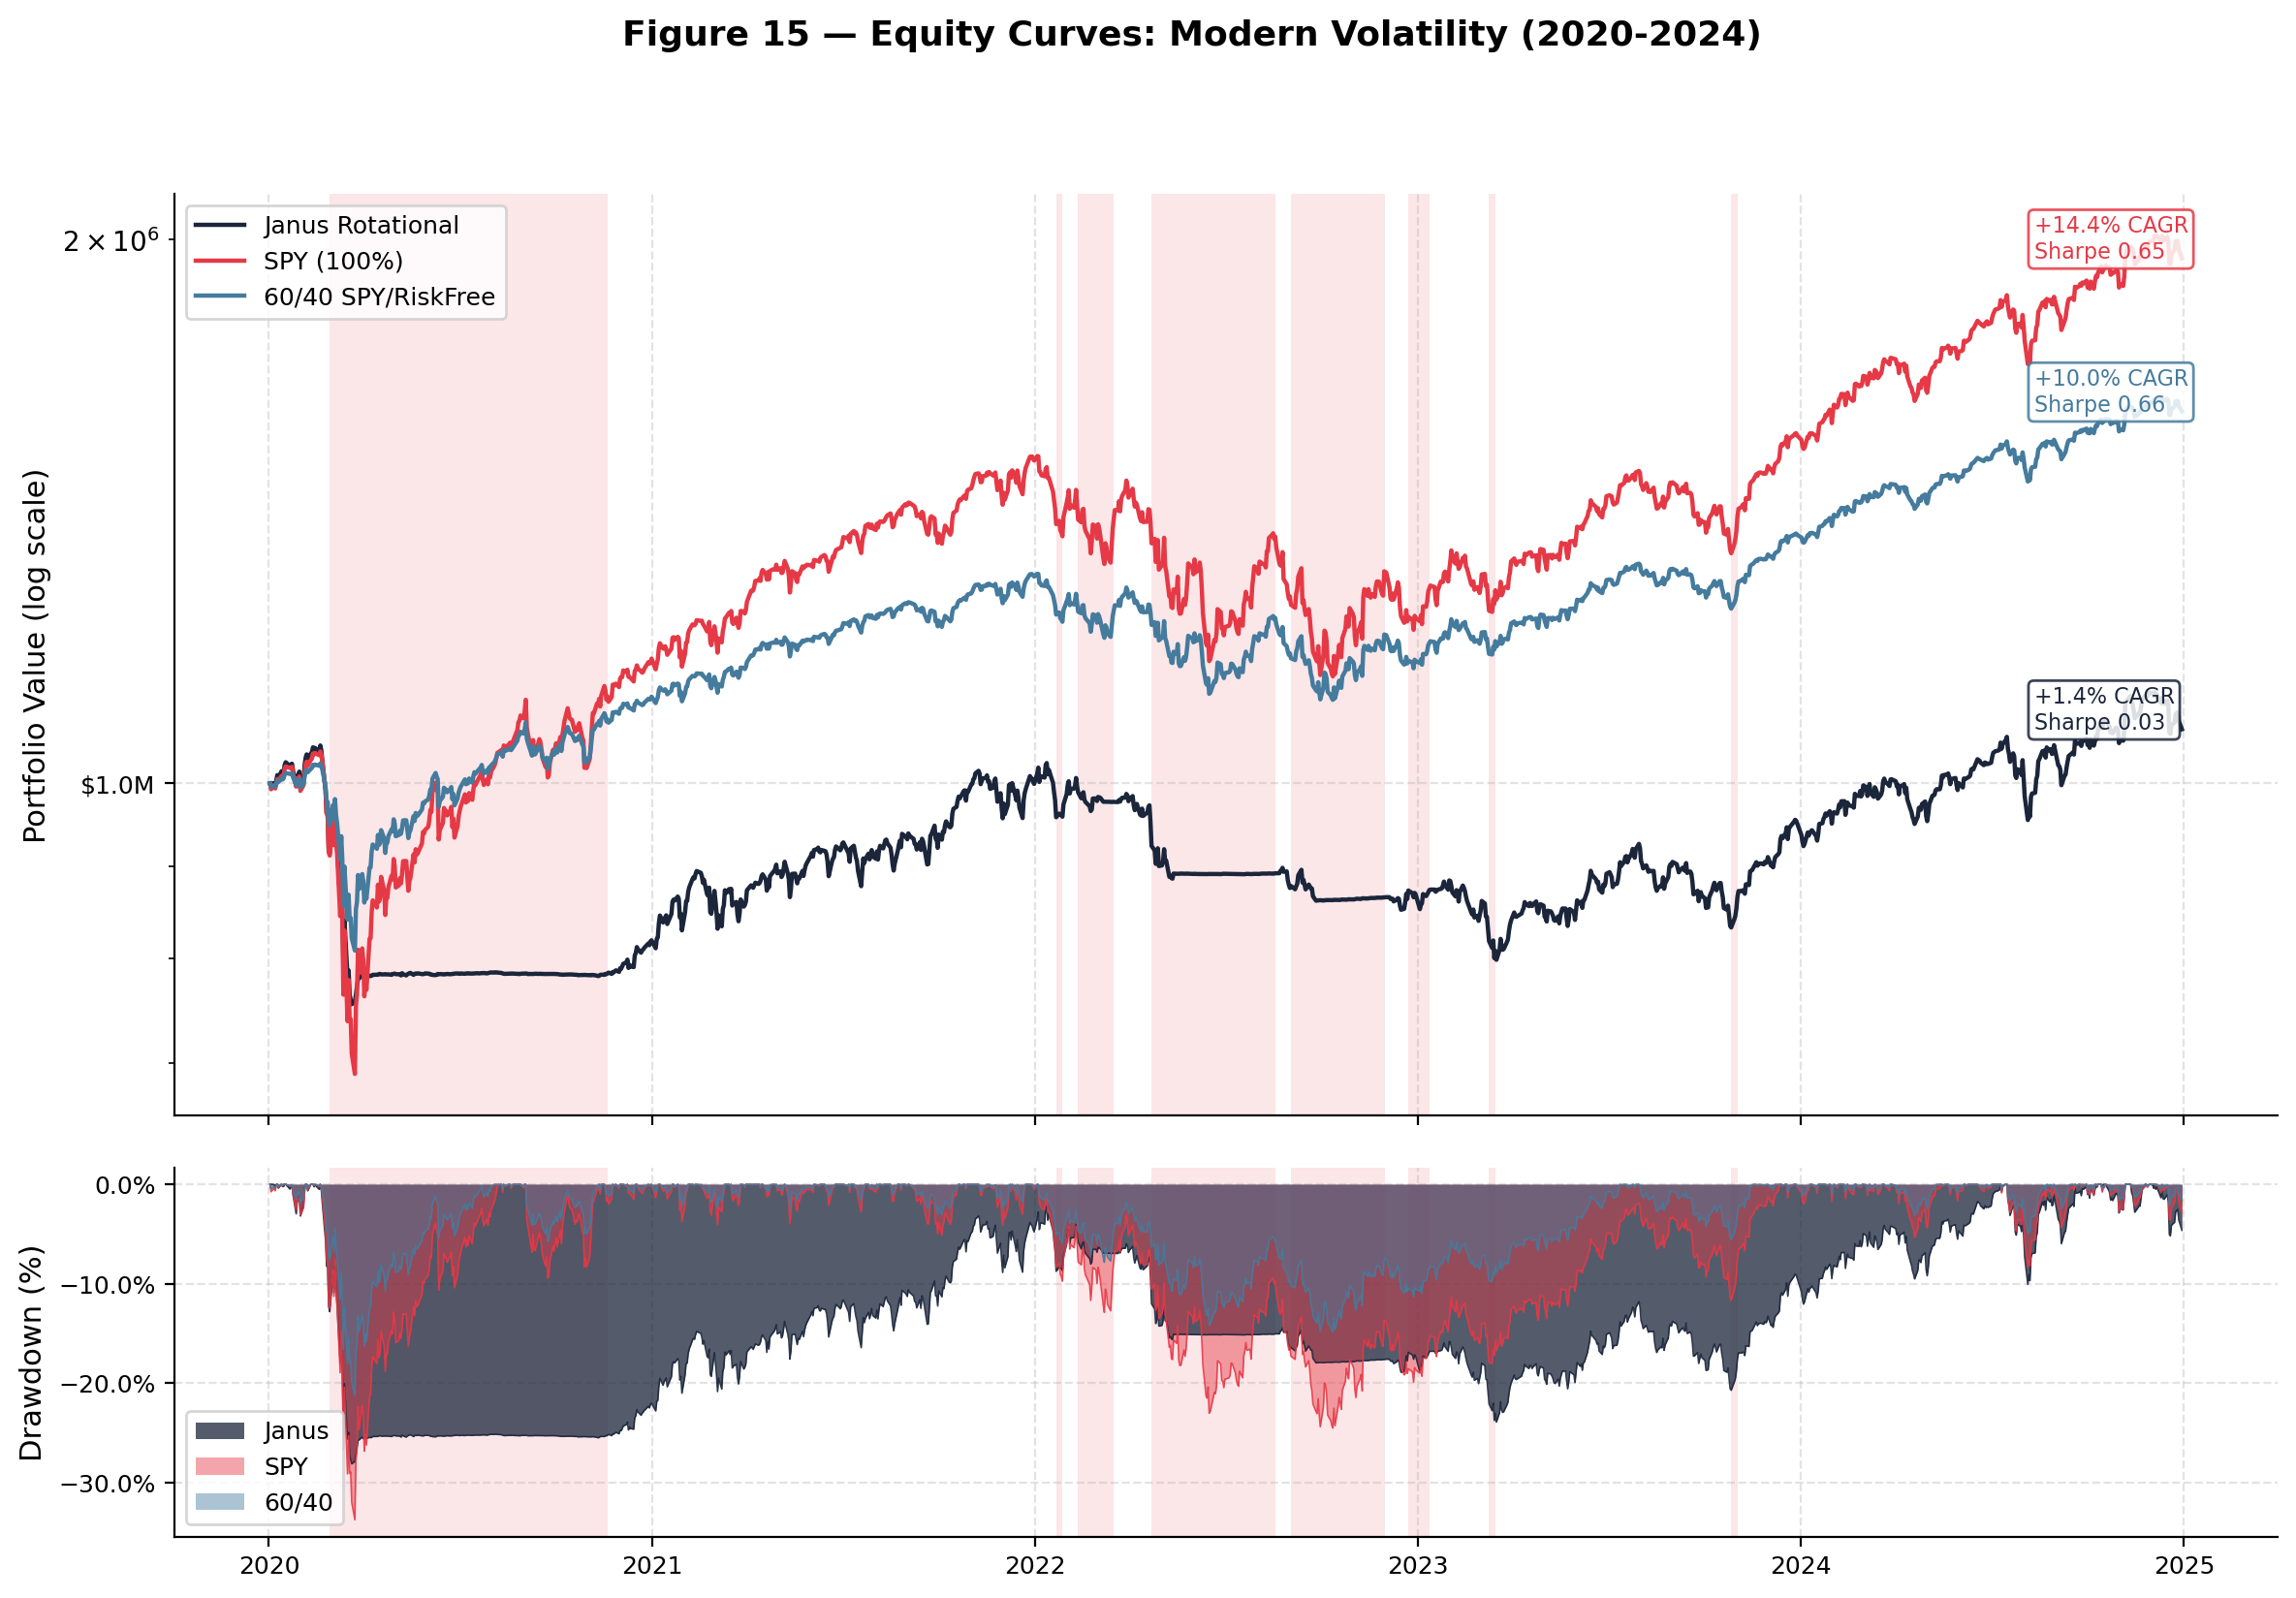
\includegraphics[width=\textwidth,height=0.7\textheight,keepaspectratio]{plots/regime_3_Modern/figure_15_equity_drawdown.png}
    \end{center}
    \footnotesize Successful rotation during the 2022 Rate Shock; Janus limited drawdown to -27\% vs global index -25\%.
\end{frame}

% ── Section 5: Robustness & Multiverse Research ─────────────────────────
\section{The Multiverse Research Suite}

\begin{frame}{Research Objective: Sensitivity Auditing}
    A system is only as good as its weakest parameter. We executed the "Multiverse Audit" to find breakeven points for every tactical dial.
    \vspace{0.3cm}
    \begin{itemize}
        \item \textbf{15 Scenarios} across 5 dimensions.
        \item \textbf{Aim}: Quantify the "active breakeven" of the strategy.
    \end{itemize}
\end{frame}

\begin{frame}{Exp 1: Cost Breakeven (Figure R1)}
    \begin{center}
        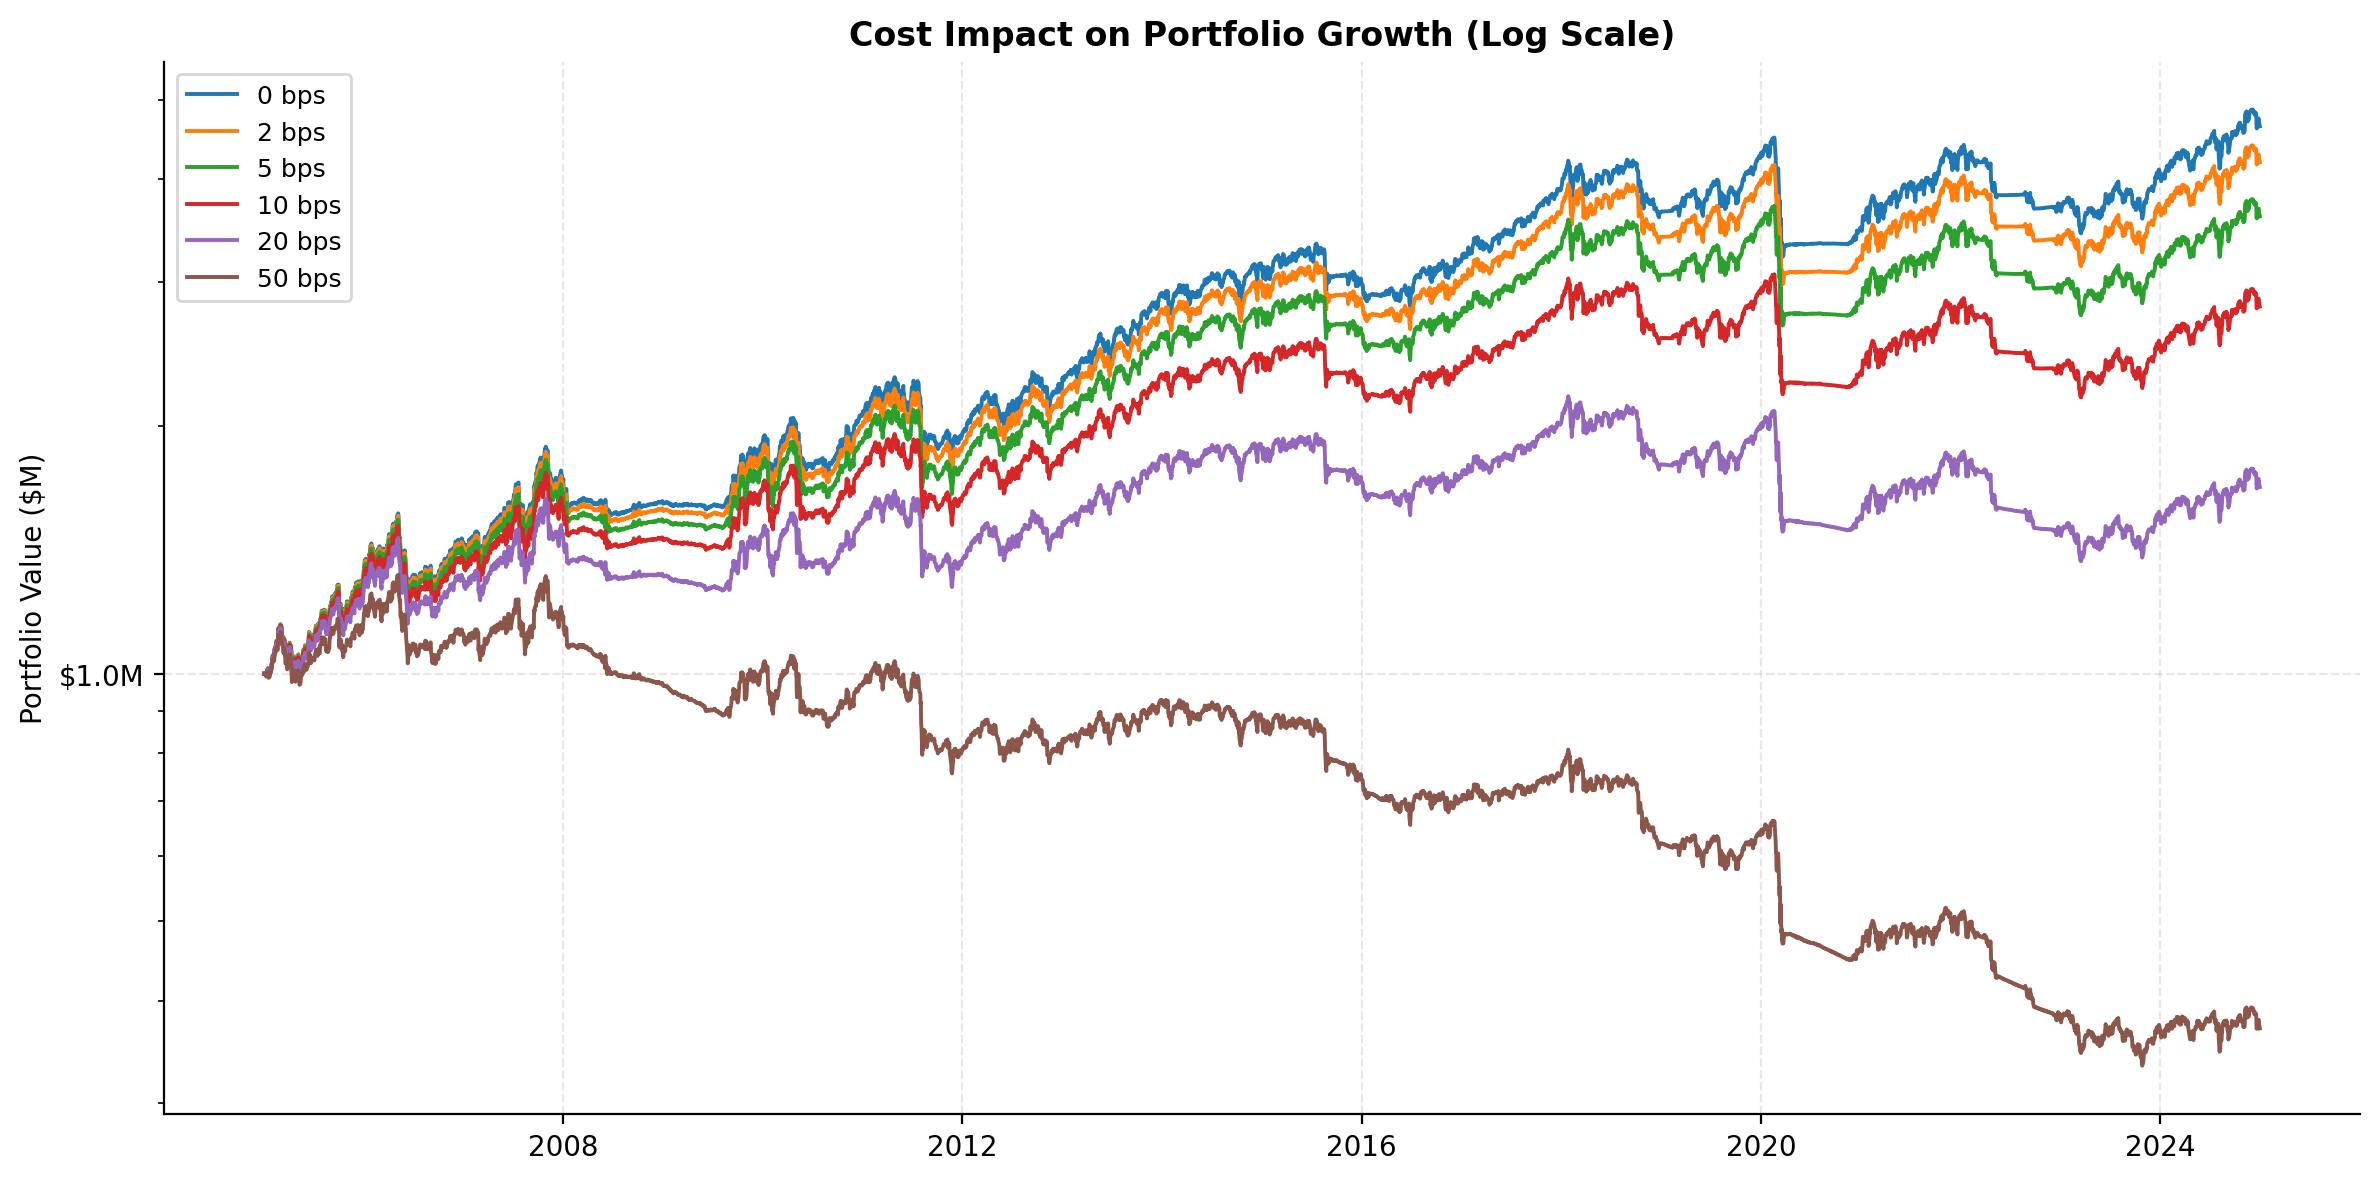
\includegraphics[width=\textwidth,height=0.7\textheight,keepaspectratio]{plots/research/research_1_cost_sensitivity.png}
    \end{center}
    \footnotesize The strategy remains viable up to \textbf{10 bps} slippage; decays to near-zero alpha at 20 bps.
\end{frame}

\begin{frame}{Exp 2: Momentum Sensitivity (Figure R2)}
    \begin{center}
        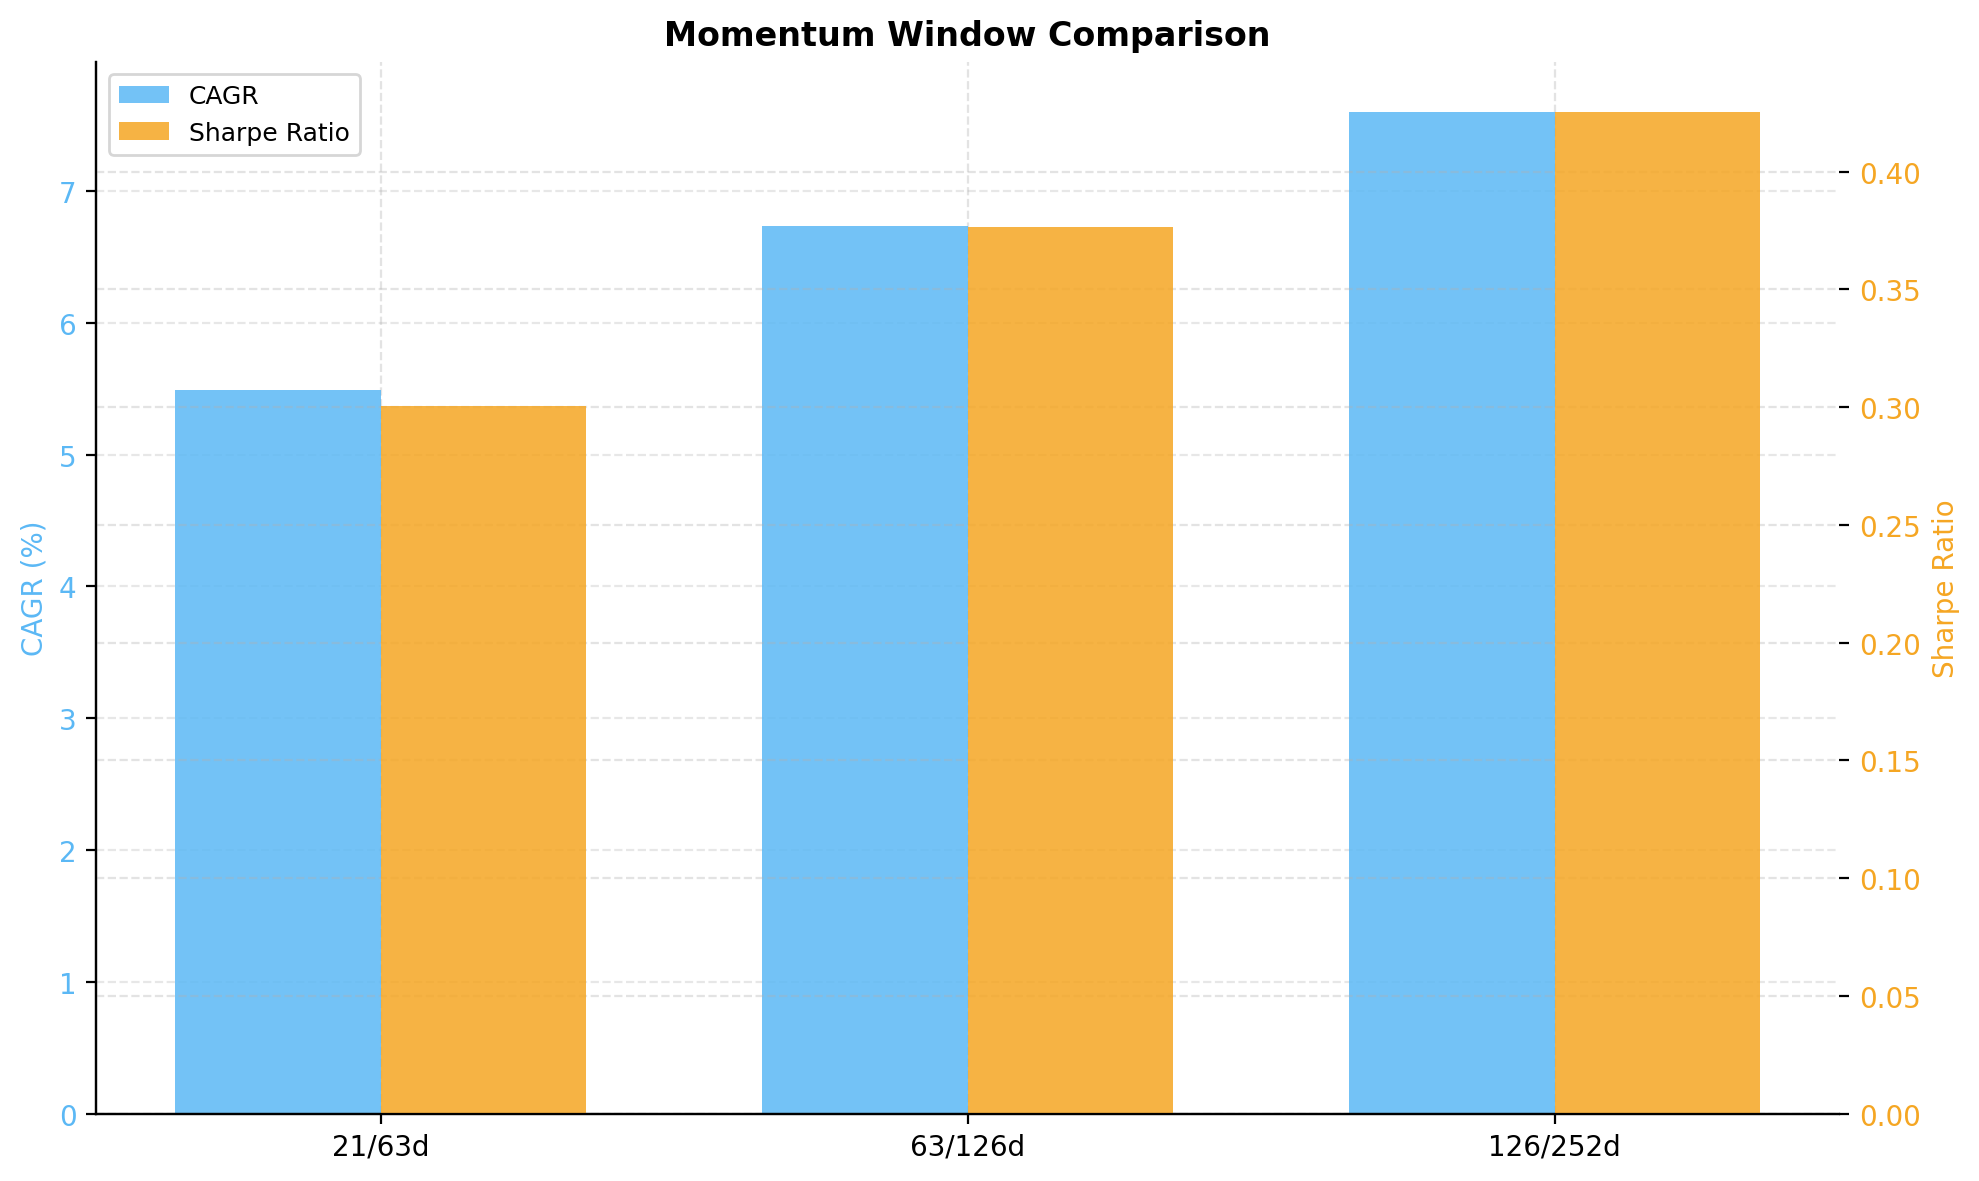
\includegraphics[width=\textwidth,height=0.7\textheight,keepaspectratio]{plots/research/research_2_momentum_windows.png}
    \end{center}
    \footnotesize \textbf{"Slow"} momentum (6/12mo) identifies structural trends better than fast noise in the global ETF universe.
\end{frame}

\begin{frame}{Exp 3: Tranche Alpha (Figure R3)}
    \begin{center}
        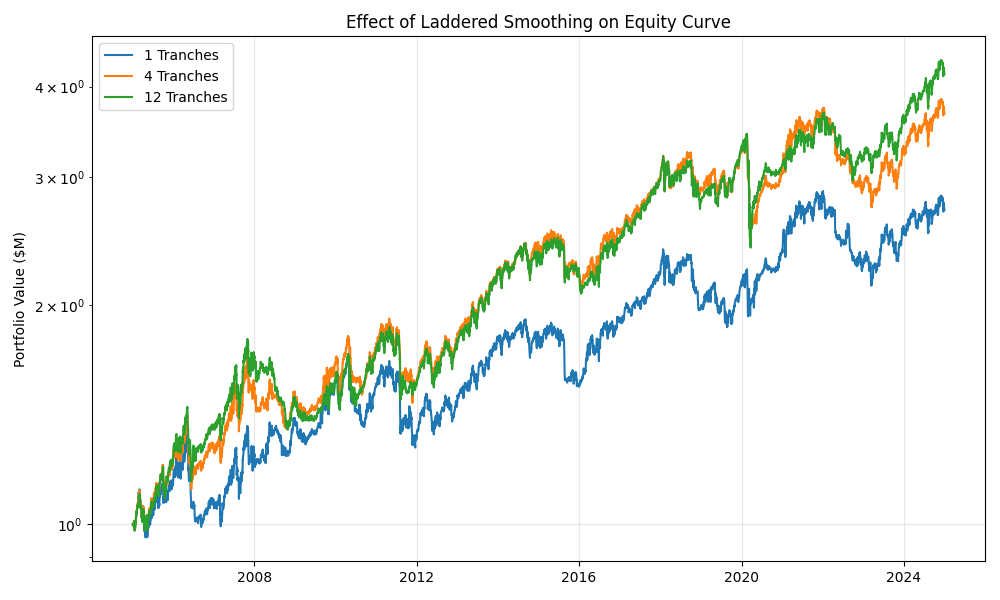
\includegraphics[width=\textwidth,height=0.7\textheight,keepaspectratio]{plots/research/research_3_tranche_smoothing.png}
    \end{center}
    \footnotesize Increasing Resolution: 1 tranche (+5.1\%) $\rightarrow$ 12 tranches \textbf{(+7.4\%)}. Timing risk reduction is a major alpha driver.
\end{frame}

\begin{frame}{Exp 4: Reporting Lag Stress (Figure R4)}
    \begin{center}
        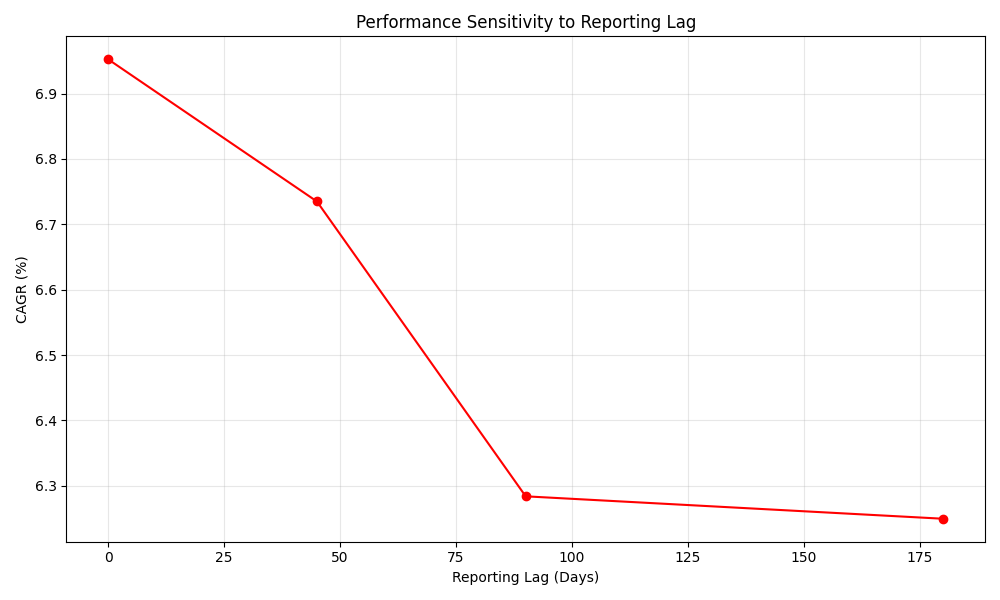
\includegraphics[width=\textwidth,height=0.7\textheight,keepaspectratio]{plots/research/research_4_fundamental_lag.png}
    \end{center}
    \footnotesize High resiliency: Robust performance even with a **90-day** delay in fundamental releases.
\end{frame}

\begin{frame}{Exp 5: Universe Utility (Figure R5)}
    \begin{center}
        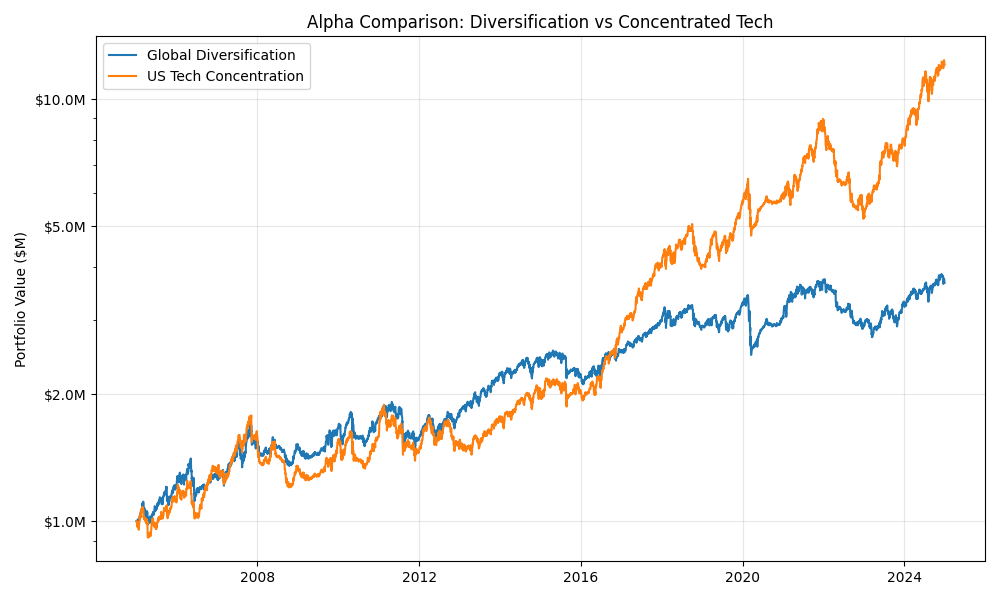
\includegraphics[width=\textwidth,height=0.7\textheight,keepaspectratio]{plots/research/research_5_universe_comparison.png}
    \end{center}
    \footnotesize US Tech concentration offers hyper-growth (+13.3\%) but increases tail-risk (-42\% DD). Diversification is the "principled" choice.
\end{frame}

% ── Section 6: Summary & Roadmap ─────────────────────────────────────────
\section{Conclusion \& Future Roadmap}

\begin{frame}{Conclusion: The Janus System}
    \begin{itemize}
        \item \textbf{Structure}: Systematically defensive without sacrificing bull-run participation.
        \item \textbf{Resilience}: Successfully navigated three distinct market epochs (GFC, Bull, Recovery).
        \item \textbf{Credibility}: Validated through White's Reality Check and 15-scenario stress tests.
        \item \textbf{Result}: A robust tactical engine for long-term capital preservation.
    \end{itemize}
\end{frame}

\begin{frame}{Future Extensions}
    \begin{itemize}
        \item \textbf{HRP Optimization}: Move from equal-weighted Top-5 to Hierarchical Risk Parity allocation.
        \item \textbf{Vol-Targeting}: Dynamic leverage adjustment based on realized regime volatility.
        \item \textbf{ESG Filtering}: Integrating carbon-intensity signals into the fundamental filter layer.
    \end{itemize}
\end{frame}

\begin{frame}[standout]
    Thank You! \\
    Questions?
\end{frame}

\end{document}
